\chapter{General Guidelines for Optimizing the Physical Data Layout and Query Processor in GDBMSs}
\label{c:guidelines}

In this section, we review the primary components that form the storage layers of \gls{gdbms}s, the system's primary operators, and the general data access patterns of these operators when evaluating a query. We then draw a basic set of guidelines that will instruct the design of the physical data layout and query-processing techniques introduced in later chapters.

Section \ref{sec:property-graph-data-model} briefly describes the \emph{property graph data model}. Section \ref{sec:storage-components} describes the primary storage components of \gls{gdbms}s that adopt the property graph data model, while Section \ref{sec:operators} reviews the query processing operators in \gls{gdbms}s. We end the chapter by stating our guidelines in Section \ref{sec:guidelines}.

\section{Property Graph Data Model}
\label{sec:property-graph-data-model}

\begin{figure}
	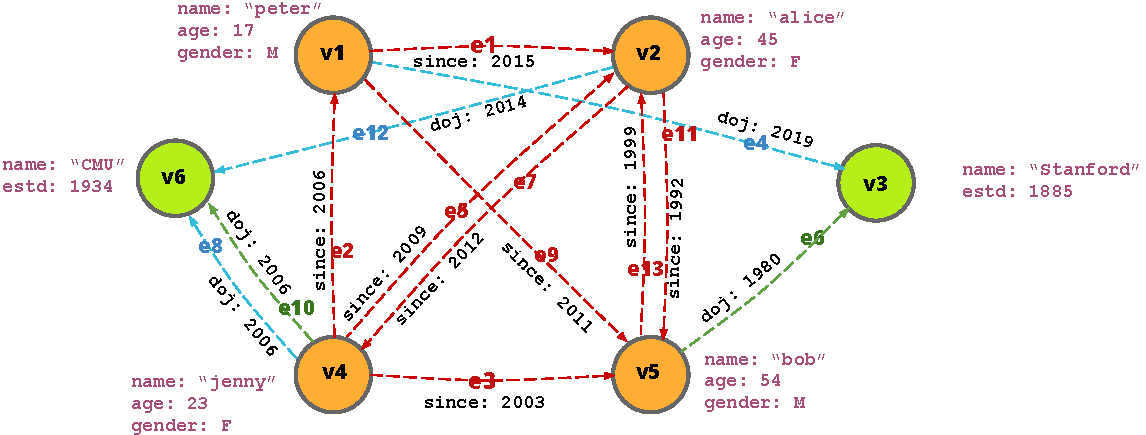
\includegraphics[scale=0.86]{img/property-graph}
	\vspace{-8pt}
	\caption{Running example graph.}
	\label{fig:runn}
	\vspace{-8pt}
\end{figure}

A property graph consists \emph{vertices} that represent entities and directed \emph{edges} between vertices that represent relationships between entities. Each vertex and edge has a particular \emph{label}, describing the high-level categories of vertices and edges. Similar to columns in relational tables, vertices and edges can have (key, value) \emph{properties}. Although the properties of vertices and edges do not need to adhere to a strict \emph{schema }, in practice many of these properties will be highly structured, i.e., similar set of properties will exist on vertices and edges of the same label.

Figure~\ref{fig:runn} shows an example graph data in property graph data model having vertex labels \texttt{PERSON} and \texttt{ORG}, and edge labels \texttt{FOLLOWS}, \texttt{WORKAT} and \texttt{STUDYAT}. 

\section{Primary Storage Components in GDBMSs}
\label{sec:storage-components}

In every \gls{gdbms} we are aware of, the edges of a graph are stored in data structure called \emph{adjacency lists}. An adjacency list of a vertex is a map to a vertex's direct set of \emph{adjacent} edges and \emph{neighbouring} vertices. In a \gls{gdbms}, each vertex has 2 adjacency lists - a \emph{forward adjacency list} containing outward edges of that vertex, and a \emph{backward adjacency list} that holds inward edges of the vertex. One can think of edges in the graph as a relational table, having 3 attributes, a source vertex, a destination vertex and an \texttt{edgeID}. The adjacency lists can then be thought of as an \emph{index} on this relational table that is \emph{clustered} by either the source or destination vertex. In practice, often this index has depth of 1 or 2, so given a vertex, a system can access its list of edges in 1 or 2 lookups. By having adjacency lists of a vertex $u$ in either direction, the system can access the list of outward and inward edges and neighbouring vertices of $u$ directly in a constant-time lookup operation, which provides the core capability of fast joins to a \gls{gdbms}. 

Typically, a single-directional adjacency list of vertex $u$ is further clustered into sublists by the edge label of the edges. This enables extending a vertex through its edges with a \emph{particular} label in constant time. The rationale behind the sub-clustering is that many queries by applications have specific label on query edges. Some systems further order the edge in the adjacency lists by either 


Moreover, the edges in a list are often ordered by either the \texttt{edgeID} or by some property of the edge or neighbouring vertex \cite{a+indexes}. Since each edge appears only once in a single-directional adjacency list, all the edges are strictly ordered in the adjacency lists.

A \gls{gdbms} also stores properties that appear on the vertices and the edges. There are multiple solutions for storing properties. The most straightforward approach is to store properties in a \emph{key-value store} \cite{dgraph} and referenced by the attribute key and the \texttt{vertexID} or \texttt{edgeID}. Properties can also be stored as a \emph{variable-sized} byte-encoded record of each vertex or edge in the same manner as row-oriented \gls{rdbms} stores tuples. A record is considered variable-sized because the number of properties on an entity is not fixed. Searching for a property in variable-sized records involves decoding and parsing the entire record until the matching attribute is found, which can be very slow. Also, the addition and deletion of properties are not straightforward in records. Yet another way of storing properties is in a doubly linked-list, as in Neo4j \cite{neo4j}, that makes additions and deletions easy though searching is still a linear-time operation.

\section{Query Execution in GDBMSs}
\label{sec:operators}

In this section, we review the general execution of queries in a \gls{gdbms} by analyzing major operators used in the query plans. Though systems differ in their architectures and implementation of operators that they support, there is still a 

We use the Cypher query language \cite{cypher} to describe the queries to a \gls{gdbms}.  A user query $Q$ typically consists of 2 parts, 
a subgraph pattern $G$ that is matched against the graph topology, and a conjunctive set of predicates $(P_0, P_1 ...)$ over properties of query edges and vertices that the matched subgraph must satisfy. Example \ref{ex:cypher-example} shows a typical query written in Cypher language.

\vspace{-4pt}
\begin{example}
	\label{ex:cypher-example}
	Consider the following query Q. 
	{\em 
		\begin{lstlisting}[numbers=none,  showstringspaces=false,belowskip=0pt ]
		MATCH (a:PERSON)$-$[e:WORKSAT]$\rightarrow$(b:ORG)
		WHERE a.age $>$ 22 AND b.established < 2015
		RETURN *\end{lstlisting}
	}
	This query returns all the PERSON vertices and their workplaces, constrained to the condition that the \textsc{\char13}age\textsc{\char13} property of PERSON vertex has a value that is greater than 22 and \textsc{\char13}established\textsc{\char13} property of ORG vertex is less than 2015. a and b are query vertex variables while e is a query edge variable.
\end{example}
\vspace{-5pt}

Query execution in GDBMS is \emph{volcano-styled}, that is, the query subgraph pattern is matched on the graph and evaluated one match at a time. The following are the major operators used for matching the subgraph pattern and evaluating predicates in a query.
\begin{itemize}
	
	\item \textbf{\texttt{SCAN}}: \texttt{Scan} is the first operator of any query plan that matches a single query vertex to all the eligible vertices in the graph and passes their \texttt{vertexID} to the next operator in the query plan. The output of the \texttt{SCAN} operator is a partially matched subgraph to the query's subgraph pattern $G$ which contains a singleton vertex. We call this partially matched subgraph $G_0$.
	
	\item \textbf{\texttt{EXTEND/INTERSECT (E/I)}}: The input to the \texttt{E/I} opertor is a partially matched subgraph $G_{k-1}$, where $k$ is the number of matched query vertices. This operator matches the next query vertex variable $v$ from $G$, such that there is at least one edge, in \emph{any} direction, between $u$ and $G_{k-1}$'s vertex variables. The output is a partially matched subgraph $G_{k}$, having $G_{k-1}'s$ vertex variabels and variable $v$. 
	
	If $v$ has only a single query edge $e$ to any one of $G_{k-1}$'s vertices, say $u$, then the \texttt{EXTEND} operator is used. if $e$ is ($u\rightarrow v$), operation is called \texttt{forward EXTEND} which reads edges from the \emph{forward adjacency list} of $u$'s match, while matching $v$ to each of the neighbouring vertices in the adjacency list. \texttt{backward EXTEND} operation can be similarly inferred. $u$'s match is called the \emph{extending vertex}.
	
	If there are $\ge$ one edges, say $(e_1, e_2 ...)$, from $v$ to $G_{k-1}$'s vertex variables, such that $(e_1, e_2 ...)$ connects variables $(u_1, u_2 ...)$ in $G_{k-1}$ to $v$, then \texttt{INTERSECT} operator performs intersection of the appropriate adjacency lists of $(u_1, u_2 ...)$ and matches the common edges and neighbouring vertices.  
	
	\item \textbf{\texttt{PROPERTY READER}}: (Vertex/Edge) Property Reader reads the properties of the query vertices and edges which are required for evaluating query predicate $P$, from the underlying properties storage. 
	
	\item \textbf{\texttt{EXPRESSION EVALUATOR AND FILTER}}: The expression evaluator evaluates the expressions in the predicate $P$ of the query and filters out the matched subgraphs that do not agree to the constraints specified in the query.
	
\end{itemize}

Out of all plans generated by the query enumerator for query Example \ref{ex:cypher-example}, one of the plans exist with the follwing sequence of operations, 1) \texttt{SCAN} $a$, 2) \texttt{EXTEND} $a{\rightarrow}b$, 3) \texttt{PROPERTY READER} for $a.age$, 4) \texttt{PROPERTY READER} for $b.established$, and finally, 5) \texttt{EXPRESSION EVALUATOR AND FILTER}. Note that we ignore other operators that are responsible for storing and returning from the query.

\section{Guidelines}
\label{sec:guidelines}

We next outline a set of guidelines for designing the physical data layout and query processor of a \gls{gdbms}.

\begin{guideline}[Edges are doubly-indexed.]
Each edge appears in the forward adjacency list of that edge's source vertex and the backward adjacency list of it's destination vertex. This results in a 2x replication factor in storing the topology of a graph in the system. This  replication cannot be avoided by dropping an adjacency list in any one direction without hampering the capability to perform fast neighbour joins, which is one of the core feature of \gls{gdbms}s.
\end{guideline}

\label{ssec:edges-ordered}
\begin{guideline}[Edge properties are read in the same order as edges in an adjacency list.]
The set of edges (having relevant edge label) of the extending vertex extended can be accessed in a constant-time operation. These edges are read by the \texttt{E/I} operator in the same \emph{order} as they are stored in the adjacency list. Note that the edge might not be read in consecutive operations, hence we do not call the access \emph{sequential}; nevertheless, ordering is preserved. Furthermore, if the query is required to read some or all of the edge properties of the edges, the properties are also read in the same order in which the edges are read from the adjacency list which itself is the order in which edges are stored.

The idea of orderly reads straightaway triggers the question of whether we can read edges and edge properties sequentially from the memory at once and hence benefit from the cache locality available at hand. However, there are 2 concerns in achieving sequential access: 

\begin{enumerate}
	
	\item The edge properties should be organized in the order identical to that of edges in the adjacency list.
	
	\item For organizing edge properties in the order identical to that of edges in the adjacency list, each property has to be replicated twice, once for each of the 2 adjacency lists in the system.
	
	\item The idea of sequential reads of edges itself \emph{does not} hold much relevance with the volcano-style processing in \gls{gdbms}s, which matches the subgraph pattern in the query tuple-at-a-time.
	
\end{enumerate}

\end{guideline}

\subsection{Vertices cannot be ordered or sequentially read.}
\label{gdln:vertices-unordered}

Contrary to how the edges and edge properties can be strictly ordered for each of the adjacency lists, there cannot be any strict ordering on the vertices and its properties. This is because, in a single-directional adjacency list, a vertex can appear \textit{n} number of times as the neighbouring vertex of an extending vertex, where \textit{n} is the number of edges the neighbouring vertex has in the direction opposite to that of the adjacency lists. Moreover, concerns that exist with reading edges sequentially, are also valid for sequentially reading vertices.

\begin{guideline}[Graph data often has partial structure.]
\label{gdln:graph-schema}
Even though the property graph data model is semi-structured, in practise many graph databases stored in \gls{gdbms}s have structure in different components, which \gls{gdbms}s can exploit. One reason this structure exist is that, as observed by prior works \cite{survey}, often the data in \gls{gdbms} comes from structured data in \gls{rdbms}. Infact, several of the \gls{gdbms} providers from the industry and some academics are actively working of defining a schema language for the property graph data model \cite{schema-validation-bonifati, defining-schema-hartig}. We identify three commonly appearing structure in property graph data:

\begin{enumerate}
	
	\item Often, edge labels in the graph data have a well-defined set of source and destination vertex label(s). This restricts the vertices to  having inward or outward edges of only a definite set of labels. For example, in the LDBC social network benchmark \cite{ldbc}, edges having label KNOWS only exists between vertices of label PERSON.
	\label{gdln:graph-schema-rule1}
	
	\item The number of edges of a particular label to which a source or destination vertex can be associated, is a property of the edge label. We call this the \emph{cardinlaity} of an edge label. \emph{One-to-one} cardinality means that there can only be single edge of a particular label from a source vertex and to a destination vertex. \emph{Many-to-one} permits a single edge of a label from a source vertex but multiple edges to a destination vertex. Similar analogy can be applied to \emph{one-to-many} and \emph{many-to-many} cardinality edge labels too.
	\label{gdln:graph-schema-rule2}
	
	\item Similar to the attributes of a relational table, properties on an edge or vertex and the datatypes of these properties can \emph{often} be determined by its edge or vertex label. For example, a vertex of label PERSON in LDBC SNB has the following properties: firstName:\texttt{STRING}, lastName: \texttt{STRING}, gender:\texttt{INT} etc., that occurs on all the vertices of label PERSON. As long as a significant fraction of vertices and edges with a particular label have a common set of properties, a system can exploit this structuredness to store these properties more efficiently. 
	
\end{enumerate}

Such structure in data provides an opportunity to design more efficient and simpler data structures for accessing the storage layer of \gls{gdbms}. However, not all data in graph databases has structure. As a working terminology, we will use the following terms in this thesis:

\begin{itemize}
	\item \textbf{Structured/unstructured edge:} An edge of a particular label, that follows above-mentioned points \ref{gdln:graph-schema-rule1} and \ref{gdln:graph-schema-rule2}, is called an structured edge. An edge that is not structured, is called an unstructured edge.
	 
	\item \textbf{Structured/unstructured property:} A structured property is a property on a vertex or edge that, 1) can be determined by the vertex type or edge label of that entity; 2) appears in a significant fraction of the vertices of edges of a particular label; and 3) have the same data type in all its occurrence. Any property that is not a structured poperty, is considered unstructed.
	
\end{itemize}

We focus on optimizing the storage of structured part of the graph data in this thesis. It forms an interesting research topic to optimize a system for unstructured part of graph data. A standard approach is to serialize the key, datatype and value of each property  of our work on structured properties. Owing to the erratic nature of unstructured properties, storing them in variable-length records or linked-list as (attribute, value) pairs is a viable solution. Structured property storage can, however, be optimized to benefit memory footprint as well as access performance.

\end{guideline}

\begin{guideline}[Queries read a small subset of the vertex or edge properties]
In order to understand the nature of queries user ask on \gls{gdbms}, we conducted a survey of 100 StackOverflow questions containing openCypher queries. We focused on queries of analytical nature and discards transactional ones like insert, delete and update. We observe the following: 

\begin{itemize}
	
	\item Out of the 100 queries, 68 accessed at least one of the properties on a vertex or an edge. Of these, 61 accesses vertex properties and 13 accesses edge properties.
	
	\item Only 11 queries returned all the properties of a query edge or vertex, while 35 of them return specific properties.
	
	\item Average number of properties accessed by those queries that explicitly return a set of properties is only 1.6.
	
\end{itemize}

We can observe that conclude that vertex properties are more popularly accessed as compared to edge properties and most of the queries only access 1 or at most 2 properties.

\end{guideline}
